\section{Introduction}
In order to increase autonomous vehicle safety and optimize route planning, vehicles must be able to effectively
communicate with one another. Specifically in hazardous situations, it is critical to communicate useful data to
relevant vehicles.
One of the main challenges in fleet-level communication is the choice of a network infrastructure suitable
for the task. Wi-Fi networks are fast and cheap to deploy but have a limited range. Communication via satellites
offer an unlimited range but are very expensive to deploy. Another challenge is deciding how much effort
each car should put in trying to advertise a dangerous situation to nearby vehicles.
Even though self-driving vehicles are expected to be capable of processing a lot of information directly on-board,
network infrastructure technologies still require engineers to minimize the amount of data exchanged on shared
communication infrastructures such as cellular or Wi-Fi networks.
We are interested in finding a set of functionalities that a fleet-level communication pipeline should exhibit
such that we can improve the safety of self-driving vehicles while minimizing the impact on on-board computers
and network infrastructures.
Tests on a realistic model of a town show that our communication strategy can reduce the number of
collisions by about $\collision_ratio_reduction_perc\%$.

\begin{figure}[t]
	\vspace{0.2cm}
    \centering
    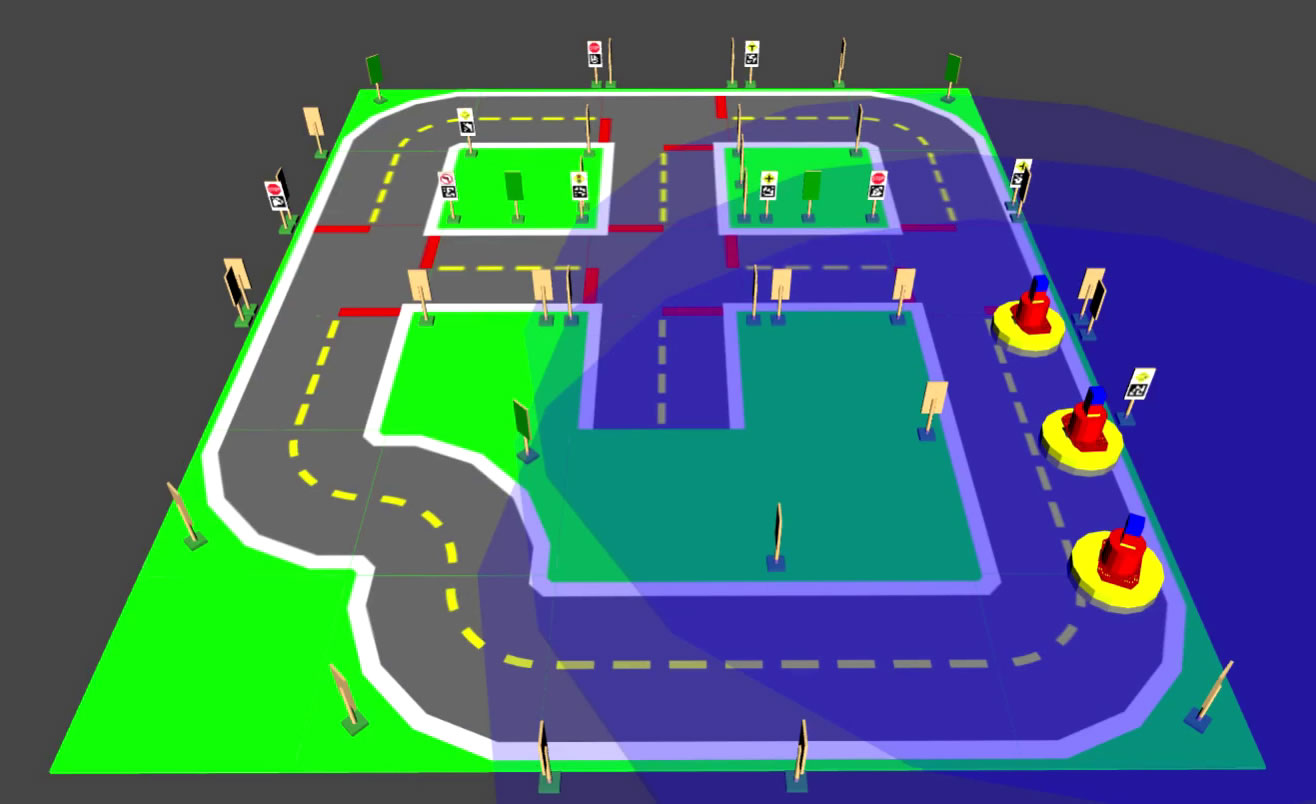
\includegraphics[width=0.48\textwidth]{figures/full-model_viewer.jpg}
    \caption{3D view of Duckietown (no simulation) showing vehicles stopping in line without colliding
    due to an accident located at the North-East 3-way intersection ($POI$).
    The \textit{yellow} circles indicate the position of the vehicles after they stopped.
    The \textit{blue} circles indicate their communication ranges. The \textit{red} cylinders
    indicate the location advertised by the vehicles as \textit{dangerous}. The small \textit{blue boxes}
    indicate that a vehicle is broadcasting messages about known dangerous locations.  \label{fig:3d_viewer_full_model}}
\end{figure}
